\documentclass[MTech]{iitmdiss}

\usepackage{times}
\usepackage{epsf}
\usepackage{threeparttable}
\usepackage{setspace}
\usepackage{amsmath}
\usepackage{gensymb}
\usepackage{amsthm}
\usepackage{txfonts,pxfonts,amsfonts}
\usepackage{epsfig}
\usepackage{caption}
\usepackage{subcaption}
\usepackage{graphicx}
% \usepackage[square,numbers,sort]{natbib}
\usepackage[square]{natbib}
\usepackage[hidelinks]{hyperref} % hyperlinks for references.
%\usepackage{algorithmic}
%\usepackage{algorithm}


%\include{commands}
\newcommand{\plt}{thesis_plots}
% Strut macros for skipping spaces above and below text in tables. 
\def\abovestrut#1{\rule[0in]{0in}{#1}\ignorespaces}
\def\belowstrut#1{\rule[-#1]{0in}{#1}\ignorespaces}

\def\abovespace{\abovestrut{0.20in }}
\def\aroundspace{\abovestrut{0.20in}\belowstrut{0.10in}}
\def\belowspace{\belowstrut{0.10in}}
%%%%%%%%%%%%%%%%%%%%%%%%%


\def\thesistitle{Motivic analysis of neuronal responses to visual stimuli}
\def\thesisauthor{Athul Vijayan}


\begin{document}
\bibliographystyle{iitm}
%%%%%%%%%%%%%%%%%%%%%%%%%%%%%%%%%%%%%%%%%%%%%%%%%%%%%%%%%%%%%%%%%%%%%% 
% Title page

\title{\thesistitle}

\author{\thesisauthor}

\date{April 2016}
\department{Engineering Design}

%\nocite{*}
\begin{singlespace}
\maketitle 
\end{singlespace} 



%%%%%%%%%%%%%%%%%%%%%%%%%%%%%%%%%%%%%%%%%%%%%%%%%%%%%%%%%%%%%%%%%%%%%%
% Certificate
\certificate

\vspace*{0.5in}

\noindent This is to certify that the thesis entitled {\bf {\thesistitle}}, 
submitted by {\bf {\thesisauthor}}, to the Indian Institute of Technology, 
Madras, for the award of the degree of {\bf Master of Technology}, 
is a bona fide record of the research work carried out by him under my
supervision. The contents of this thesis, in full or in parts, have not been
submitted to any other Institute or University for the award of any degree or
diploma.

\vspace*{1.4in}
\hspace*{-0.25in}
\begin{singlespace}
\noindent {\bf Dr.~Hema~A.~Murthy } \\
\noindent Research Guide \\ 
\noindent Assistant Professor \\
\noindent Dept. of Computer Science and Engineering\\
\noindent IIT-Madras, 600 036 \\
\end{singlespace}
\vspace*{0.20in}
\noindent Place: Chennai\\ 
Date:

%%%%%%%%%%%%%%%%%%%%%%%%%%%%%%%%%%%%%%%%%%%%%%%%%%%%%%%%%%%%%%%%%%%%%%
% Acknowledgements
\acknowledgements

**I would like to thank everyone who helped me.

%%%%%%%%%%%%%%%%%%%%%%%%%%%%%%%%%%%%%%%%%%%%%%%%%%%%%%%%%%%%%%%%%%%%%%
% Abstract
\abstract
\noindent KEYWORDS: \hspace*{0.5em} \parbox[t]{4.4in}{Markov Decision Processes,
Symmetries, Abstraction}
\vspace*{24pt}

\pagebreak
%%%%%%%%%%%%%%%%%%%%%%%%%%%%%%%%%%%%%%%%%%%%%%%%%%%%%%%%%%%%%%%%%%%%%%
% Table of contents etc.

\begin{singlespace}
\tableofcontents
\thispagestyle{empty}

\listoftables
\addcontentsline{toc}{chapter}{LIST OF TABLES}
\listoffigures
\addcontentsline{toc}{chapter}{LIST OF FIGURES}
\end{singlespace}


%%%%%%%%%%%%%%%%%%%%%%%%%%%%%%%%%%%%%%%%%%%%%%%%%%%%%%%%%%%%%%%%%%%%%%
% Abbreviations
\abbreviations
 
\noindent 
\begin{tabbing}
xxxxxxxxxxx \= xxxxxxxxxxxxxxxxxxxxxxxxxxxxxxxxxxxxxxxxxxxxxxxx \kill
\textbf{RLCS}   \> Rough Longest Common Subsequence \\
\textbf{LCSS}   \> Longest Common Segment Set \\
\end{tabbing}

\pagebreak

%%%%%%%%%%%%%%%%%%%%%%%%%%%%%%%%%%%%%%%%%%%%%%%%%%%%%%%%%%%%%%%%%%%%%%
%Notation

\chapter*{\centerline{NOTATION}}
\addcontentsline{toc}{chapter}{NOTATION}

\begin{singlespace}
\begin{tabbing}
xxxxxxxxxxx \= xxxxxxxxxxxxxxxxxxxxxxxxxxxxxxxxxxxxxxxxxxxxxxxx \kill
\textbf{$\rho(a, b)$}  \> Pearson correlation between $a$ and $b$\\
\textbf{V1}  \> Primary Visual Cortex\\
\end{tabbing}
\end{singlespace}
 
 \pagebreak
 \clearpage

\pagenumbering{arabic}


%%%%%%%%%%%%%%%%%%%%%%%%%%%%%%%%%%%%%%%%%%%%%%%%%%%%%%%%%%%%%%%%%%%%%%
\chapter{Introduction}   % 2-3 pages
\label{chap:intro}

%%%%%%%%%%%%%%%%%%%%%%%%%%%%%%%%%%%%%%%%%%%%%%%%%%%%%%%%%%%%%%%%%%%%%%
\chapter{Background and Previous work}    % 5 pages
\label{chap:lit}
\section{Visual pathway in brain} % (fold)
\label{sec:visual_pathway_in_brain}

% section visual_pathway_in_brain (end)
\section{Experiment setup} % (fold)
\label{sec:experiment_setup}
\subsection{Sinusoidal grating visual stimuli} % (fold)
\label{sub:sinusoidal_grating_visual_stimuli}

% subsection sinusoidal_grating_visual_stimuli (end)

\subsection{Natural videos visual stimuli} % (fold)
\label{sub:natural_videos_visual_stimuli}

% subsection natural_videos_visual_stimuli (end)
% section experiment_setup (end)

\section{Orientation and Directional selectivity of neurons in V1} % (fold)
\label{sec:orientation_and_directional_selectivity_of_neurons_in_v1}

% section orientation_and_directional_selectivity_of_neurons_in_v1 (end)

%%%%%%%%%%%%%%%%%%%%%%%%%%%%%%%%%%%%%%%%%%%%%%%%%%%%%%%%%%%%%%%%%%%%%%
\chapter{Analyzing neuronal properties} % 10 pages
\label{chap:searchmotif}
Characteristics of neurons in the V1 are discussed in the background section. In this chapter, we use experimental data to demonstrate the claimed properties of neurons in V1. In the experiment, a drifting sinusoidal grating video is shown to awake mice and neuronal responses were recorded. See Section~\ref{sub:sinusoidal_grating_visual_stimuli} for detailed experiment setup. 

Average response of a neuron is modeled as a function of orientation using a Gaussian function. Similarly, average response to various directions are modeled using a mixture of Gaussian functions. Root mean square of residuals are used as a goodness of fit measure.

Neurons in V1 are classified into simple, complex and unselective cells. Classifying a neuron into either of this class is useful as we can find the population of similar cells in the brain. Rather than thresholding OSI and DSI, We have used a k-means clustering algorithm with more features to classify cells.
\section{Quantifying Orientation and Directional selectivity} % (fold)
\label{sec:quantifying_orientation_and_directional_selectivity}
Modern imaging technologies allow examining responses of neurons with clarity. Even though it was known that neurons in V1 are selective to orientation, we need robust metrics to quantify degree of selectivity and preferred orientation.

Plotting responses to each stimuli direction in a vector space provides an intuition about the characteristics. In orientation space, responses of two opposite directions are averaged. Angle varies from $0\degree$ to $180\degree$ in orientation space while angle angle changes from $0\degree$ to $360\degree$ in direction space. Figure** shows responses plotted in orientation and direction space for a simple neuron. Length of the vector sum is a good metric for amount of selectivity and preferred orientation. Normalized length of vector sum in orientation space is defined as OSI(Orientation Selectivity Index).
$$OSI = \left|\frac{\sum_{k} R(\theta_k) \exp(2i\theta_k)}{\sum_{k} R(\theta_k)}\right|$$
Similarly, Normalized length of vector sum in direction space is defined as DSI(Direction Selectivity Index).
$$DSI = \left|\frac{\sum_{k} R(\theta_k) \exp(i\theta_k)}{\sum_{k} R(\theta_k)}\right|$$

Where $R(\theta_k)$ is the average response to angle $\theta_k$.\\
A simple neuron is expected to have high OSI but low DSI. Polar plots of responses in orientation and direction space is shown in Figure~\ref{fig:oridir_simple}
\begin{figure}[h]
  \begin{subfigure}[b]{0.5\textwidth}
    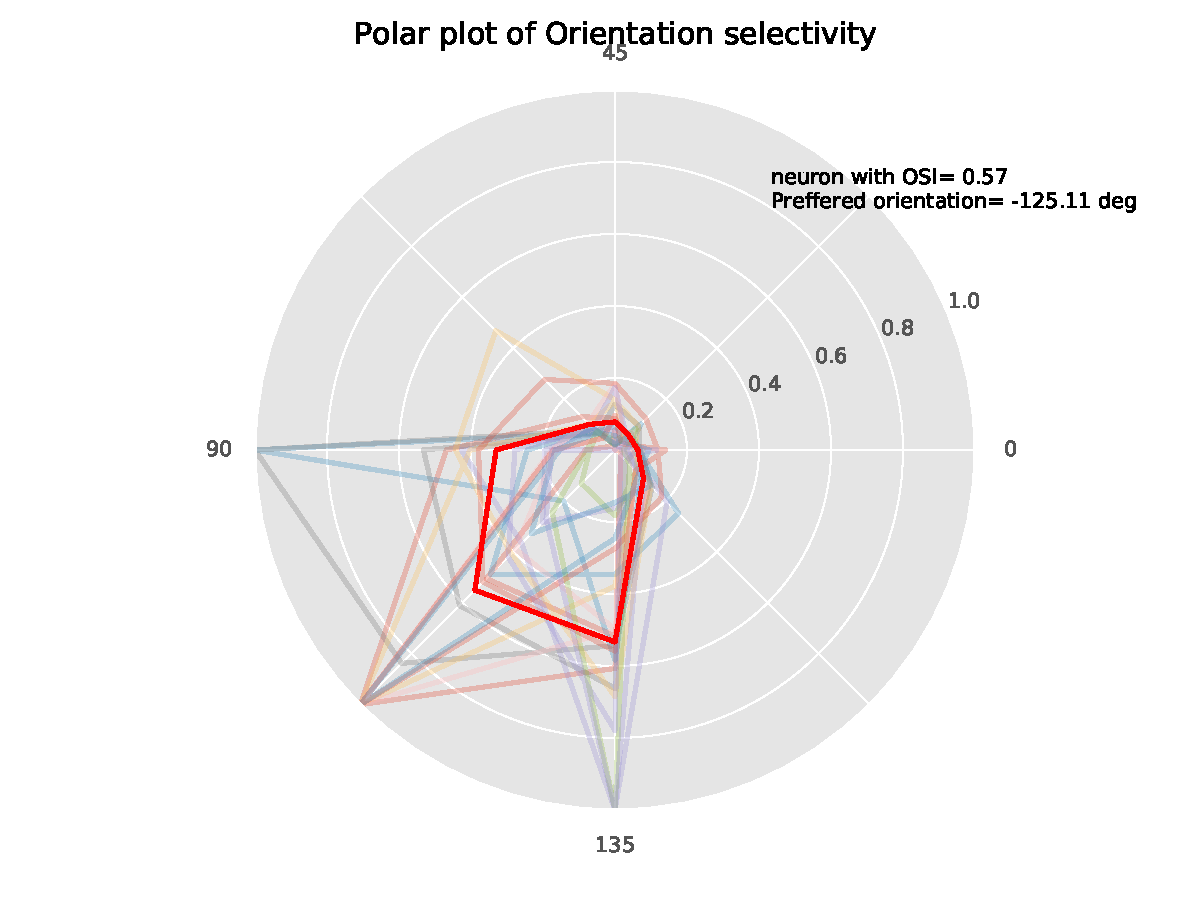
\includegraphics[width=\linewidth]{\plt/gratings_oripolar_2016_04_24_14_08_33.pdf}
    \caption{Responses plotted in orientation space}
    \label{fig:ori_simple}
  \end{subfigure}%
  \begin{subfigure}[b]{0.5\textwidth}
    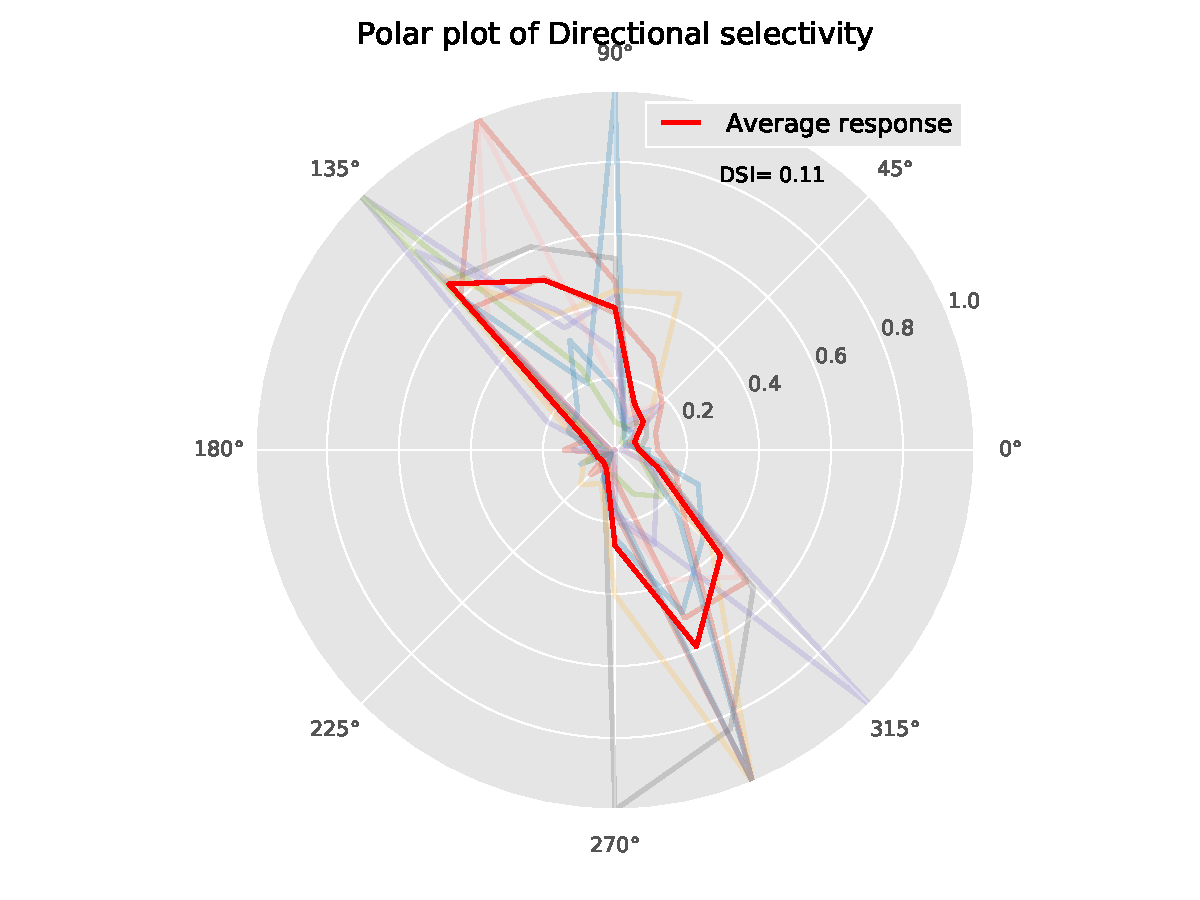
\includegraphics[width=\linewidth]{\plt/gratings_dirpolar_2016_04_24_14_08_33.pdf}
    \caption{Responses plotted in direction space}
    \label{fig:dir_simple}
  \end{subfigure}%
  \caption{Responses $R(\theta_k)$ of a simple neuron for each $\theta_k$ plotted in both orientation and direction space. Equal lobes in direction space shows direction is irrelevant.}\label{fig:oridir_simple}
\end{figure}

A complex neuron is expected to have high OSI and high DSI. Polar plots of responses in orientation and direction space is shown in Figure~\ref{fig:oridir_complex}
\begin{figure}[h]
  \begin{subfigure}[b]{0.5\textwidth}
    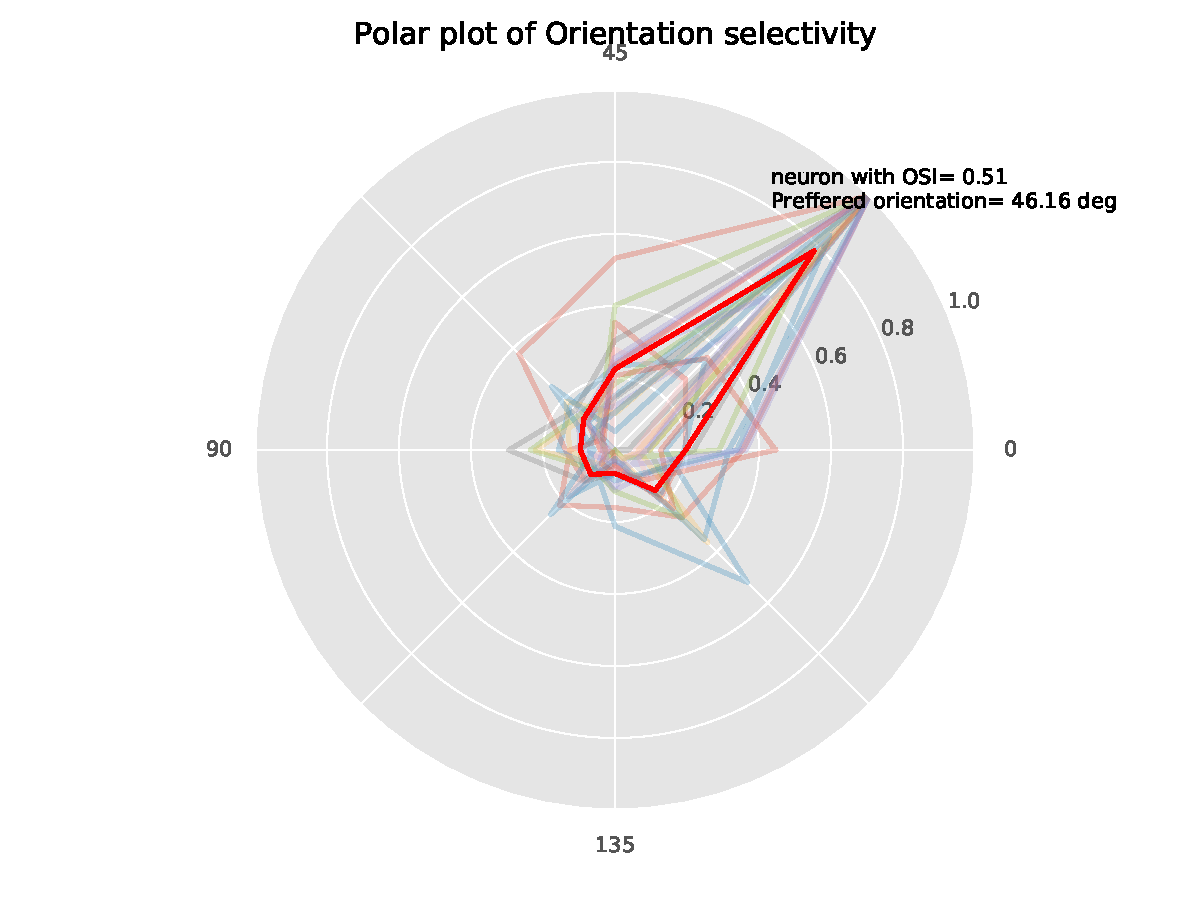
\includegraphics[width=\linewidth]{\plt/gratings_oripolar_2016_05_01_15_25_00.pdf}
    \caption{Responses plotted in orientation space}
    \label{fig:ori_complex}
  \end{subfigure}%
  \begin{subfigure}[b]{0.5\textwidth}
    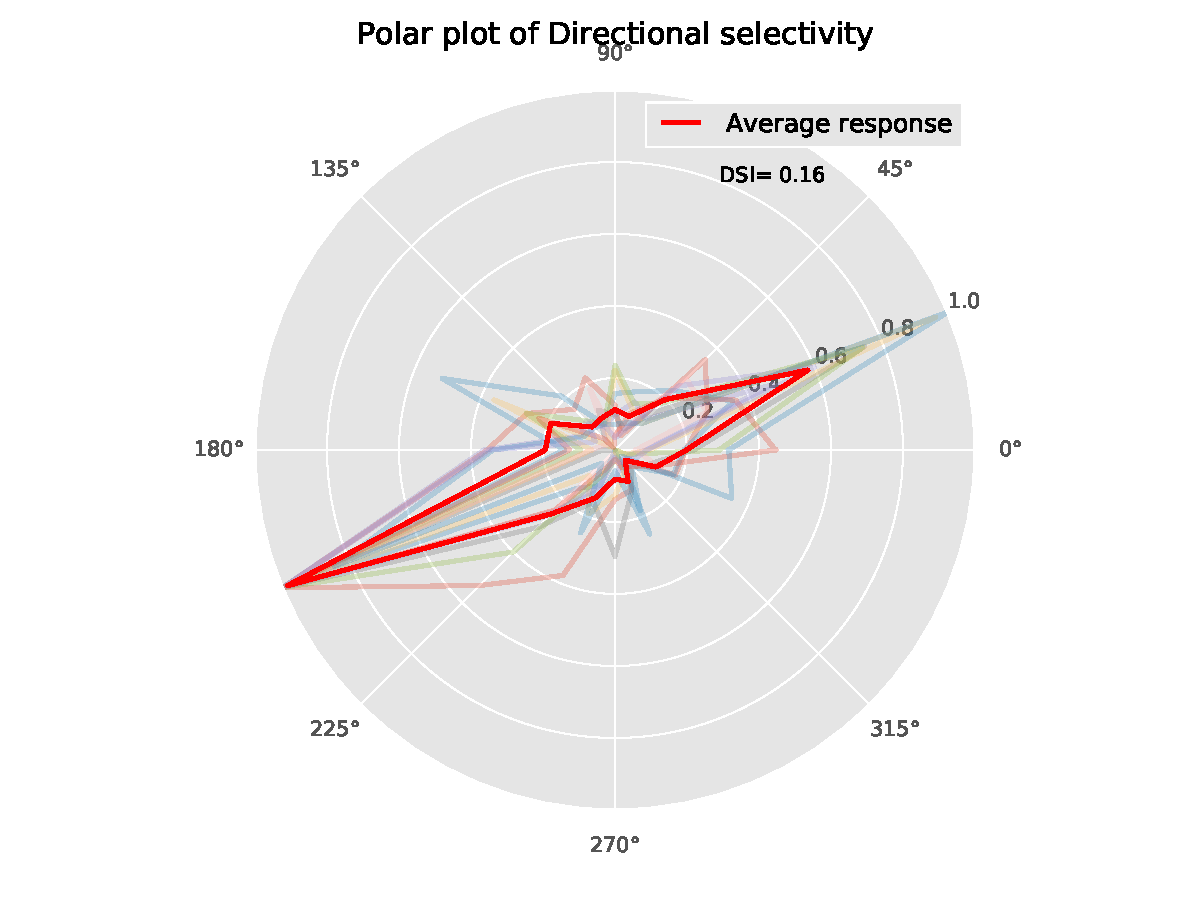
\includegraphics[width=\linewidth]{\plt/gratings_dirpolar_2016_05_01_15_25_00.pdf}
    \caption{Responses plotted in direction space}
    \label{fig:dir_complex}
  \end{subfigure}%
  \caption{Responses $R(\theta_k)$ of a complex neuron for each $\theta_k$ plotted in both orientation and direction space. Unequal lobes in direction space shows one direction is preferred than its opposite.}\label{fig:oridir_complex}
\end{figure}

An orientation insensitive neuron is expected to have low values for both OSI and DSI. Polar plots of responses in orientation and direction space is shown in Figure~\ref{fig:oridir_unsel}.
\begin{figure}[h]
  \begin{subfigure}[b]{0.5\textwidth}
    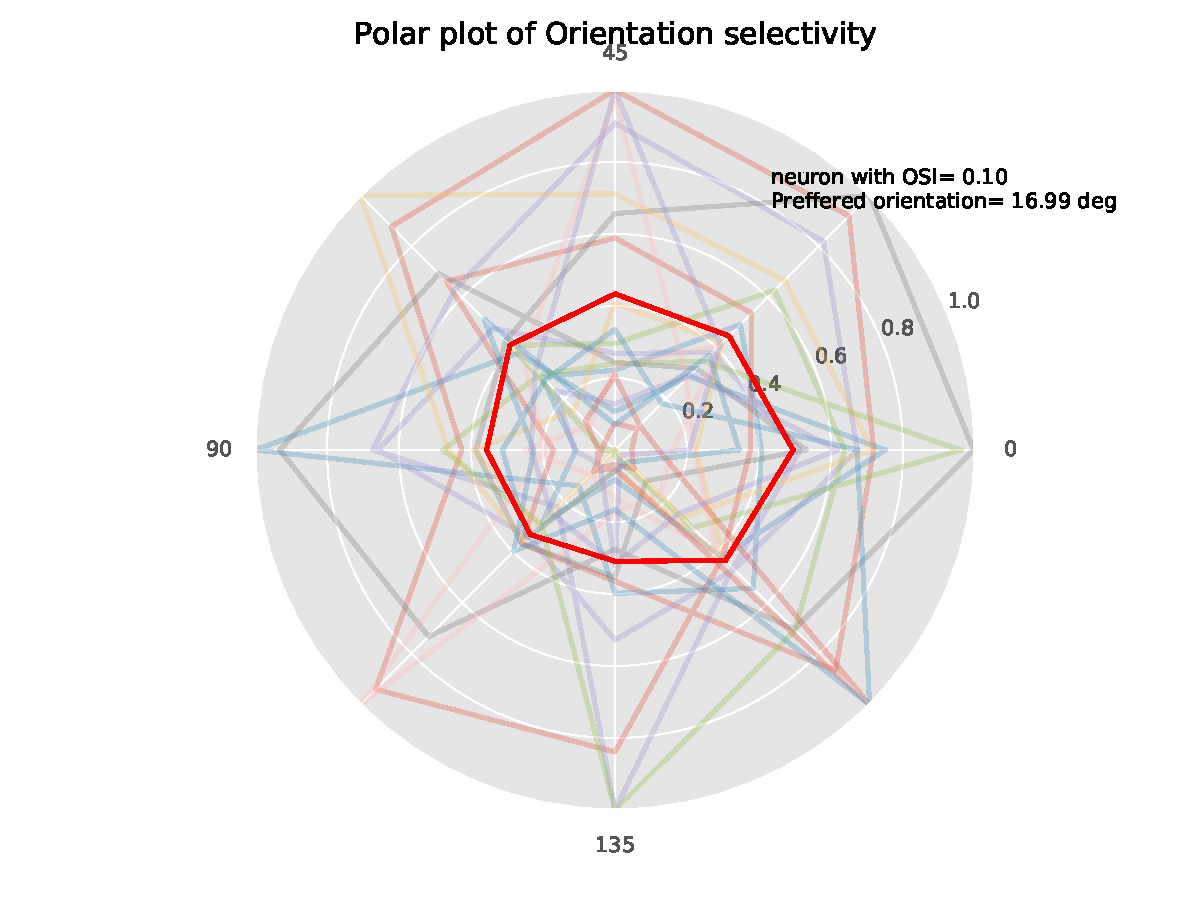
\includegraphics[width=\linewidth]{\plt/gratings_oripolar_2016_05_01_15_26_41.pdf}
    \caption{Responses plotted in orientation space}
    \label{fig:ori_unsel}
  \end{subfigure}%
  \begin{subfigure}[b]{0.5\textwidth}
    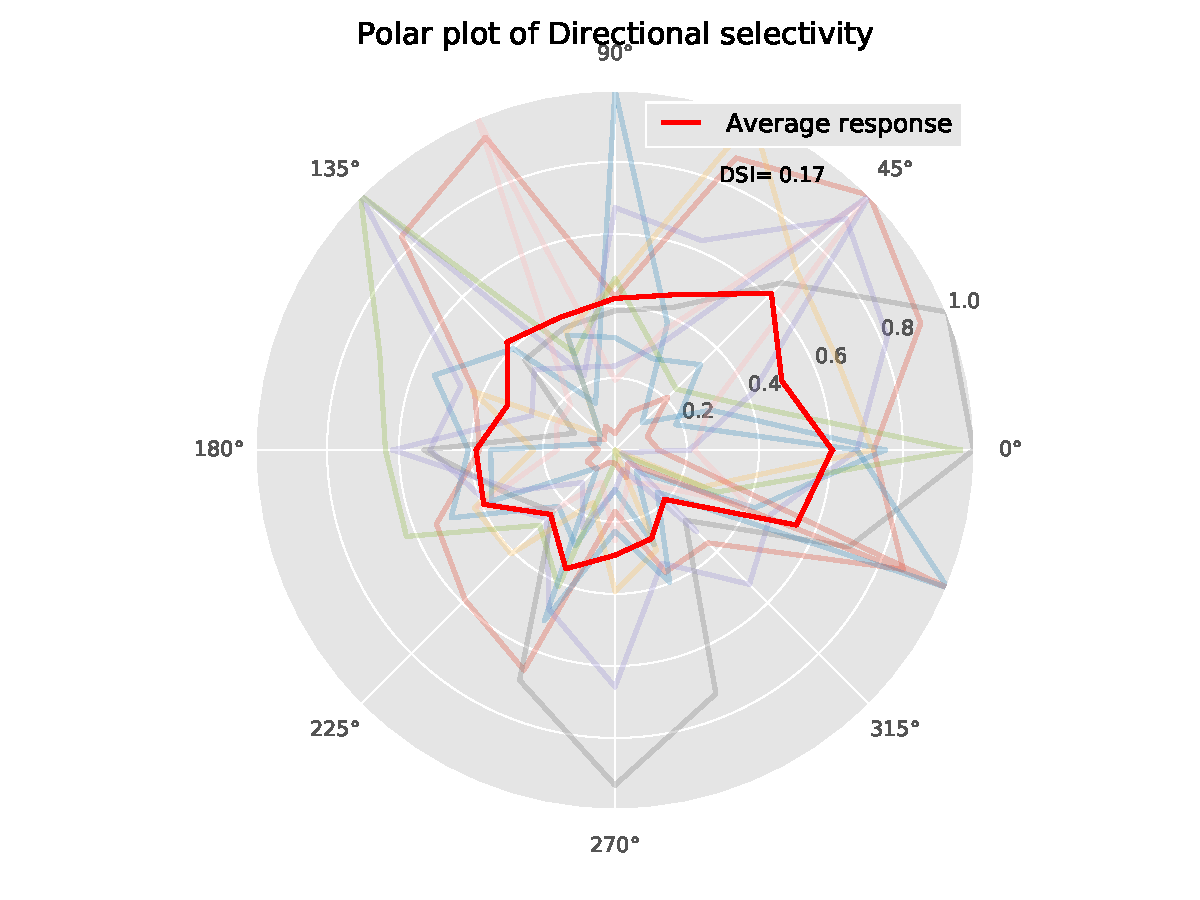
\includegraphics[width=\linewidth]{\plt/gratings_dirpolar_2016_05_01_15_26_41.pdf}
    \caption{Responses plotted in direction space}
    \label{fig:dir_unsel}
  \end{subfigure}%
  \caption{Responses $R(\theta_k)$ of a an orientation insensitive neuron for each $\theta_k$ plotted in both orientation and direction space. Similar responses to all orientations shows absence of selectivity.}\label{fig:oridir_unsel}
\end{figure}
% section quantifying_orientation_and_directional_selectivity (end)

\section{Modeling neuronal response} % (fold)
\label{sec:modeling_neuronal_response_to_sinusoidal_gratings_stimuli}
Modeling the response of neuron to various orientations and visualizing is a great way to see if in fact there is an orientation selectivity. If the cell seems selective, we can also characterize the degree of selectivity and preferred orientation from model parameters.

Orientation tuning curve is modeled using a Gaussian function with constant offset. The empirical form of the orientation tuning curve is,
$$R_o(\theta) = C + R_p \exp\left\{\frac{-||\theta-\theta_{pref}||^2}{2\sigma^2}\right\}$$
Where $R_o(\theta)$ is the time-averaged response of neuron to angle of orientation $\theta$. Parameter $\theta_{pref}$ is the preferred orientation of the neuron. Tuning width $\sigma$  tell us how much the cell is selective. $C$ is a constant offset.

Similarly, we can model direction tuning curve using a mixture of Gaussian functions with a constant offset. 
$$R_d(\theta) = C + R_p \exp\left\{\frac{-||\theta-\theta_{pref}||^2}{2\sigma_1^2}\right\} + R_n \exp\left\{\frac{-||\theta-\theta_{null}||^2}{2\sigma_2^2}\right\}$$
Where $R_o(\theta)$ is the time-averaged response of neuron to angle of direction $\theta$. Relative magnitude of tuning widths, $\sigma_1$ and $\sigma_2$ denote the amount of directional selectivity. $C$ is a constant offset.
% section modeling_neuronal_response_to_sinusoidal_gratings_stimuli (end)

Parameters are estimated by minimizing squared sum of error. Sum of squared error is defined as:
$$SSE = \sum_{i=1}^N ||R(\theta_i) - R_o(\theta_i)||^2$$
A gradient descent algorithm finds the optimum parameters by minimizing SSE.
In Figure~\ref{fig:curvefit_complex} , fit of tuning curves of a complex cell is given. The distinct peak in the orientation tuning curve shows selectivity to orientation $\theta_{pref}$. In the direction tuning curve, peaks of different magnitude shows one direction is more preferred than other.
\begin{figure}[h]
  \begin{subfigure}[b]{0.5\textwidth}
    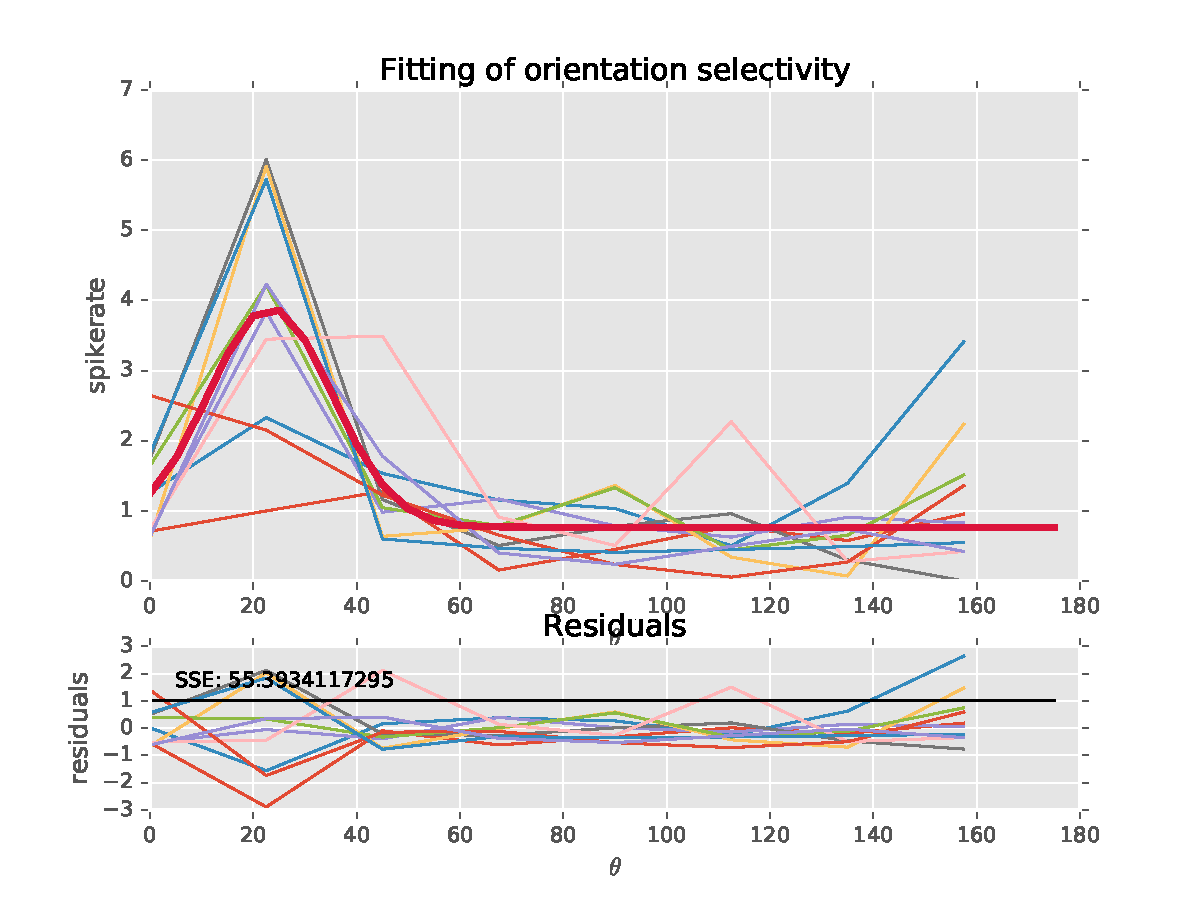
\includegraphics[width=\linewidth]{\plt/gratings_crvefit_osi_n_3_2016_05_02_12_53_03.pdf}
    \caption{Orientation tuning curve}
    \label{fig:oritune_complex}
  \end{subfigure}%
  \begin{subfigure}[b]{0.5\textwidth}
    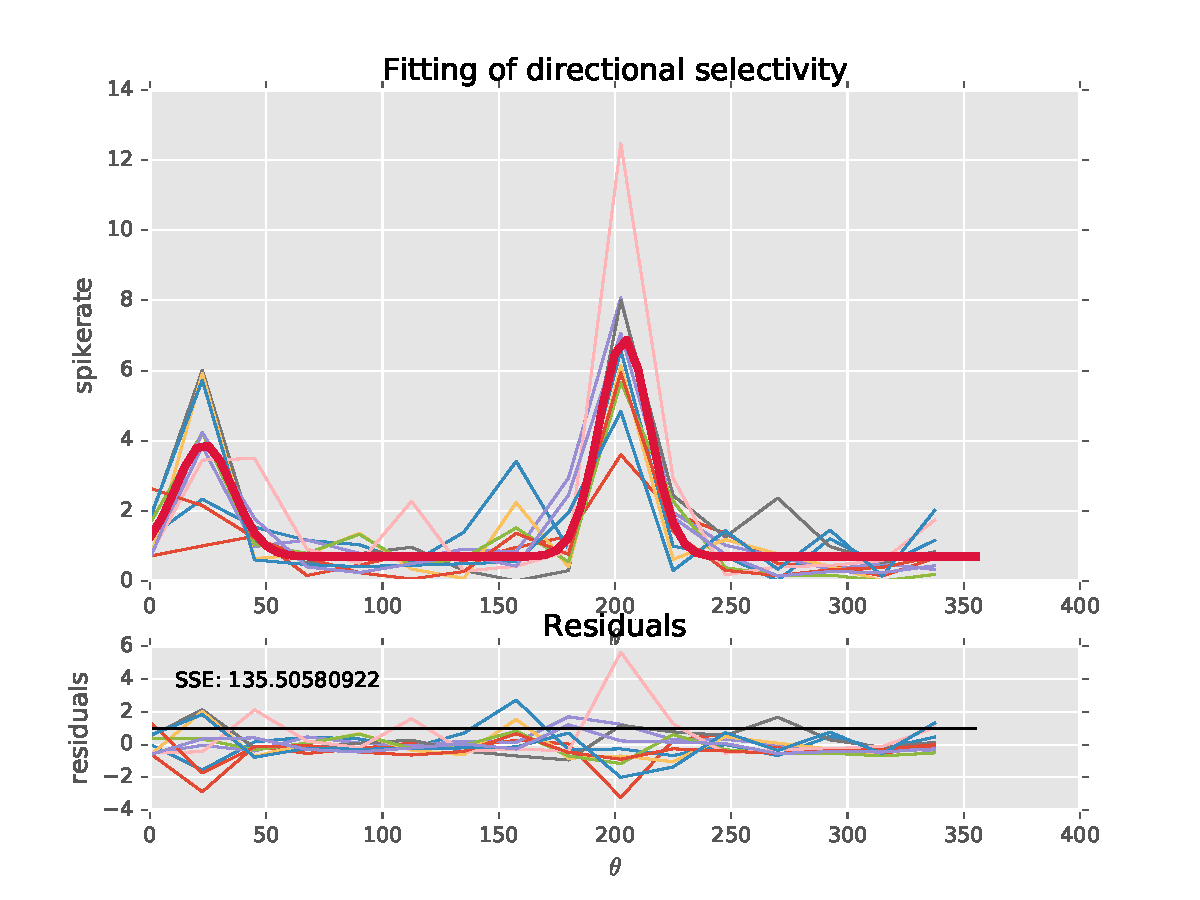
\includegraphics[width=\linewidth]{\plt/gratings_crvefit_n_3_2016_05_01_15_40_28.pdf}
    \caption{Direction tuning curve}
    \label{fig:dirtune_complex}
  \end{subfigure}%
  \caption{Fit of orientation and direction tuning curves of a neuron. The distinct peak in the orientation tuning curve shows selectivity to orientation $\theta_{pref}$. Different $\sigma_1$ and $\sigma_2$ in direction tuning curve shows direction sensitive cell. - Thus a complex cell}\label{fig:curvefit_complex}
\end{figure}
In Figure~\ref{fig:curvefit_simple} , fit of tuning curves of a complex cell is given. The distinct peak in the orientation tuning curve shows selectivity to orientation $\theta_{pref}$. In the direction tuning curve, peaks of same magnitude shows of stimuli direction is irrelevant.
\begin{figure}[h]
  \begin{subfigure}[b]{0.5\textwidth}
    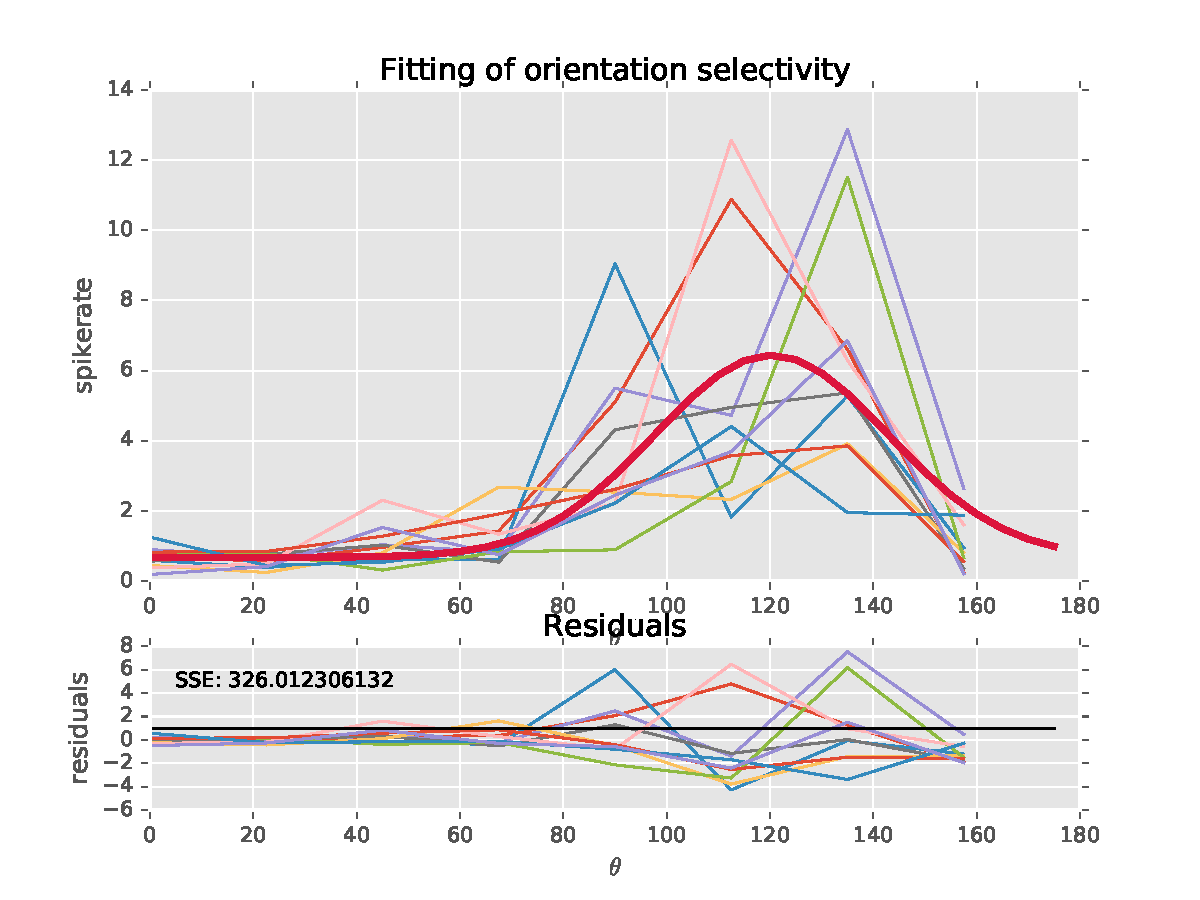
\includegraphics[width=\linewidth]{\plt/gratings_crvefit_osi_n_0_2016_05_02_12_52_43.pdf}
    \caption{Orientation tuning curve}
    \label{fig:oritune_simple}
  \end{subfigure}%
  \begin{subfigure}[b]{0.5\textwidth}
    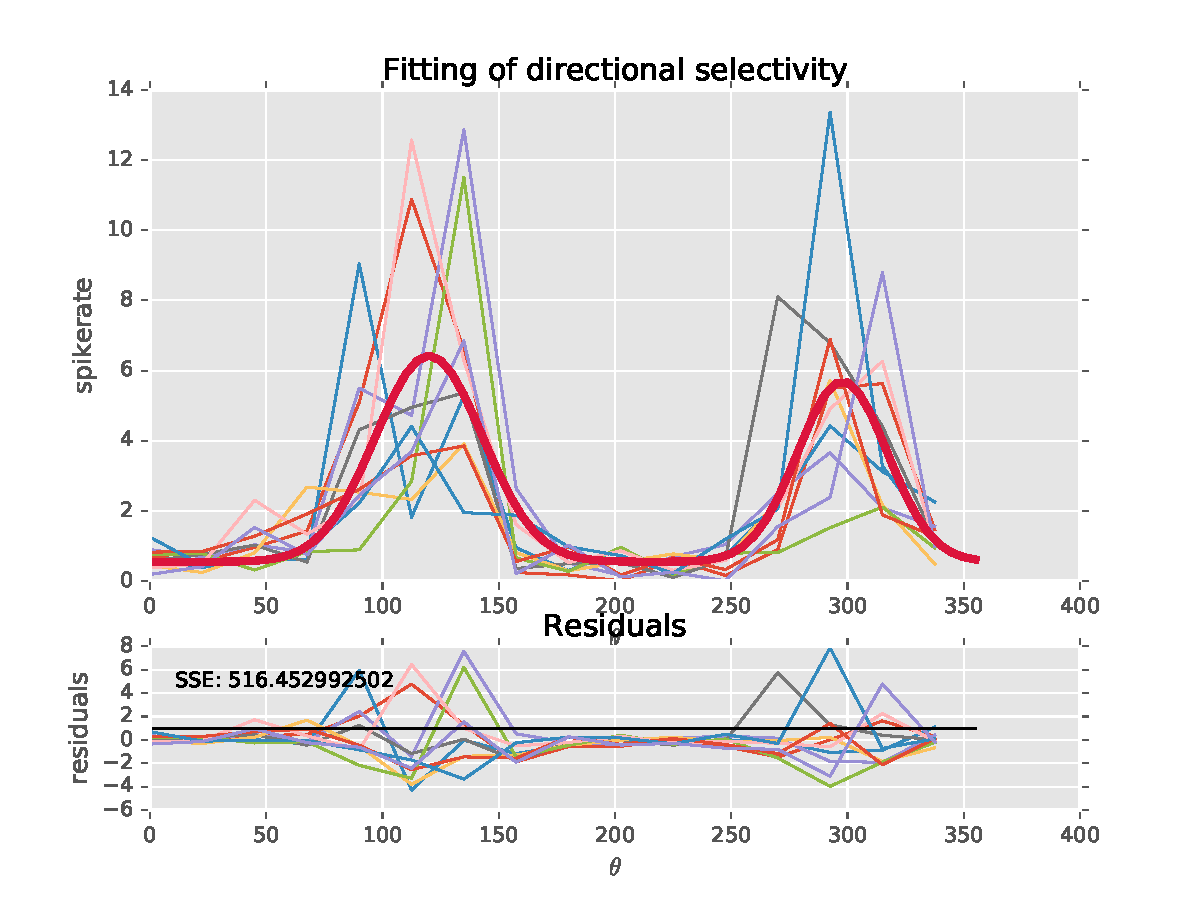
\includegraphics[width=\linewidth]{\plt/gratings_crvefit_n_0_2016_05_01_15_40_26.pdf}
    \caption{Direction tuning curve}
    \label{fig:dirtune_simple}
  \end{subfigure}%
  \caption{Fit of orientation and direction tuning curves of a neuron. The distinct peak in the orientation tuning curve shows selectivity to orientation $\theta_{pref}$. Similar $\sigma_1$ and $\sigma_2$ in direction tuning curve direction of stimuli is irrelevant. - Thus a simple cell}\label{fig:curvefit_simple}
\end{figure}
\section{Finding similarly tuned neurons} % (fold)
\label{sec:finding_similarly_tuned_neurons}
Receptive field of a neuron in V1 consists of a subset of neurons in one layer below it. Those neurons in turn have a receptive field. By following layers down, we can find a visual field for each neuron in V1. Orientation selectivity of neurons in V1 detects edges and their orientation in images. By studying similarly tuned neurons, we can get an insight to redundancy of coding and distribution of functionally similar cells in V1.

Similarly tuned cells are expected to have similar response to different stimuli orientations. A high correlation of responses $R(\theta_k)$ to various angle $\theta_k$ will represent similarly tuned cells. Even after having same preferred orientations, the neurons could have different degree of selectivity. We would like to find similarly tuned neurons which have an `acceptable' OSI.

Pearson correlation between each pair of neurons in a mice are computed and plotted in Figure~\ref{fig:corr}. The neurons in both axes have a decreasing OSI value. The neuron pairs that lei in bottom left of the Figure~\ref{fig:corr} are the ones we have interested. Finally to find neurons that are similarly tuned to a particular neuron, choose the corresponding row and all the neurons in that row having good correlation value and having acceptable OSI are selected. Figure~\ref{fig:tunecurves} shows tuning curves of some neurons retrieved from correlation study.
\begin{figure}[h]
  \centering
  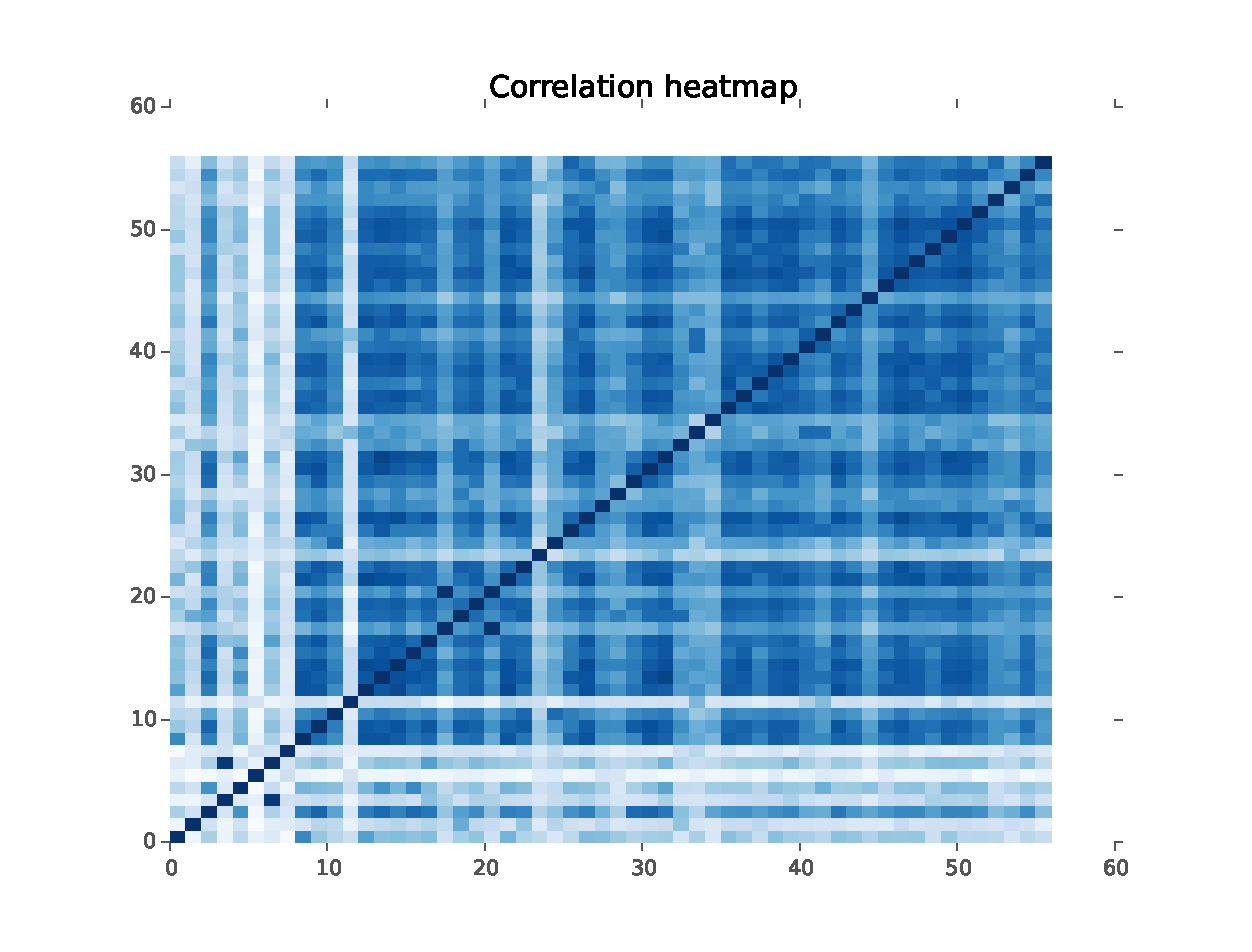
\includegraphics[width=.9\linewidth]{\plt/tuningCorr_desc_civar_m2}
  \caption{Pairwise Pearson correlation of neurons. Both axes are sorted in decreasing order of OSI.}
  \label{fig:corr}
\end{figure}
\begin{figure}[h]
  \centering
  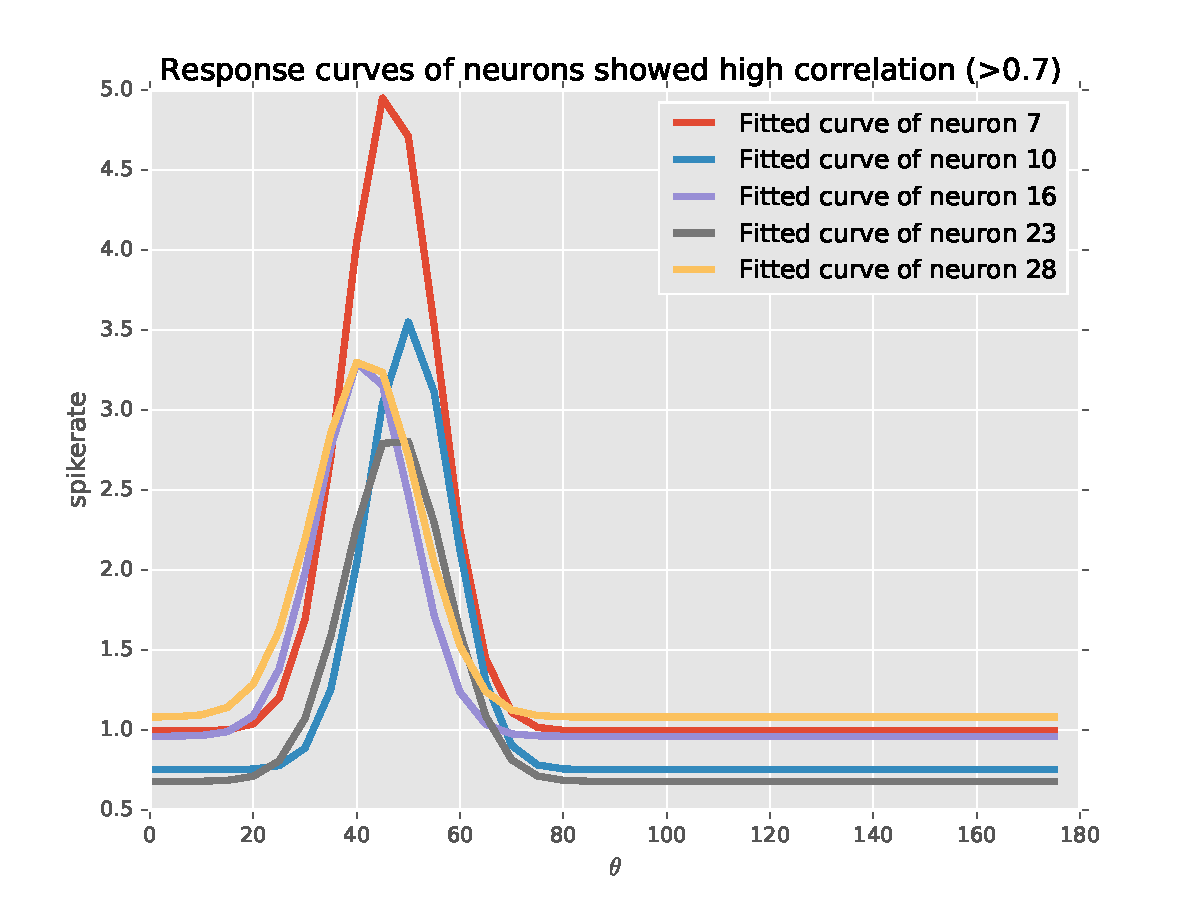
\includegraphics[width=.9\linewidth]{\plt/gratings_sel_model_2016_05_02_15_57_20.pdf}
  \caption{Orientation tuning curves of some neurons retrieved from correlation study. All of them have a same preferred orientation.}
  \label{fig:tunecurves}
\end{figure}

\section{Study of principal components} % (fold)
\label{sec:study_of_correlation}
Information contained in the visual stimuli reaches V1 after it gets passed through lower layers. Edges and motion of edges in the stimuli are represented by orientation and direction sensitive neurons in V1. Through Principal Component Analysis (PCA) we aim to study the tightness of information representation. A subset of neurons ($\sim 60$) in V1 are sampled at 20Hz for 6 seconds during the experiment. We analyze principal components of the responses to find redundancy in the responses. The number of uncorrelated principal components which capture `most' of the variance in data can determine redundancy.

Principal Component Analysis is an orthogonal transformation of possibly correlated observations to linearly uncorrelated components called principal components.  The principal components are orthogonal because they are the eigenvectors of the covariance matrix, which is symmetric. The first principal component captures largest variance and decreases further. By observing number of components that needs to capture a desired variance, we can tell correlations in the data. Transforming original data to new orthogonal basis gives a representation which has dimension less than or equal to the number of original dimension. Reconstructing original data from subset of principal components also indicates amount of correlation in original data.

Here we take number of neurons as feature dimension. The responses are averages across trials.  PCA is done on the data to find ratio between number of principal components and variance explained. Figure~\ref{img:pca} shows the result for a mouse towards a sinusoidal grating stimuli. The original data was transformed to principal components basis with a subset of principal components. Attempting to reconstructing original data from transformed data produces an error. The reconstruction error depends on number of chosen subset of principal components. Figure shows reconstruction error for different number of principal components. As we increase number of principal components, the error decreases. And finally as the number components equals the original feature dimension, reconstruction error vanish.

\begin{figure}
    \centering
    \begin{subfigure}[b]{.48\textwidth}
        \centering
        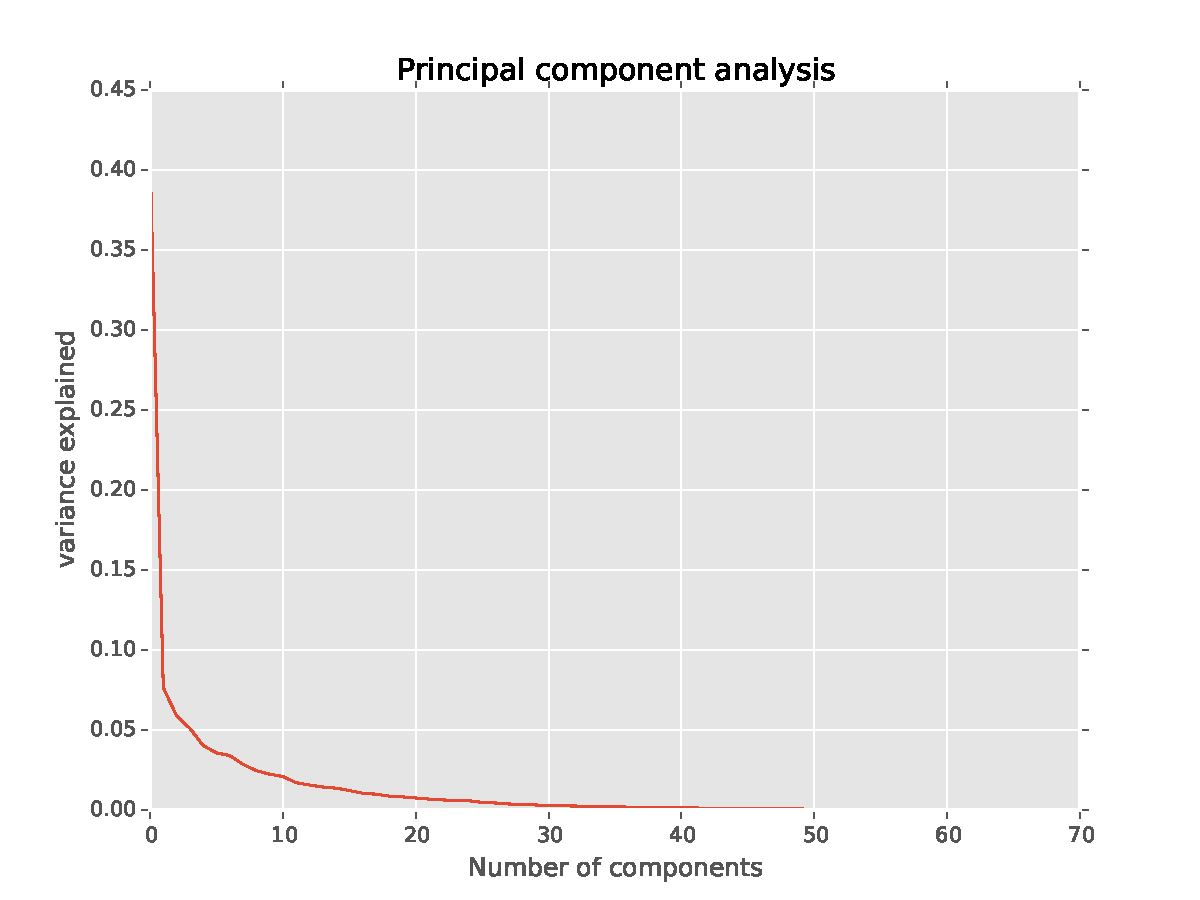
\includegraphics[width=\linewidth]{\plt/subsetbMain_pcaPlot_2016_02_05_15_41_05.pdf}
        \caption{Variance captured by components}
        \label{img:pca}
    \end{subfigure}
    ~
    \begin{subfigure}[b]{.48\textwidth}
        \centering
        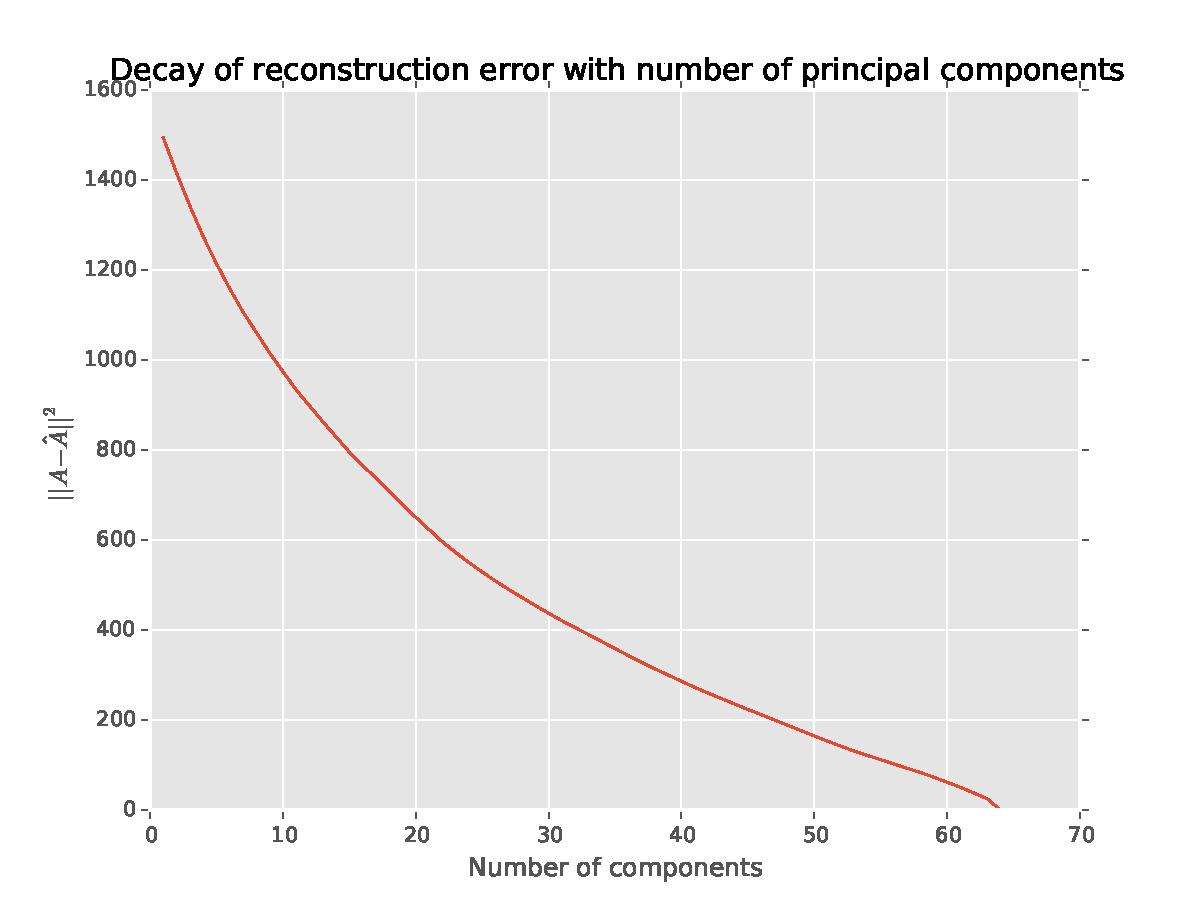
\includegraphics[width=\linewidth]{\plt/subsetbMain_errPlot_2016_02_12_12_42_39.pdf}
        \caption{Decay of reconstruction error}
        \label{img:reconstruction}
    \end{subfigure}
    \caption{Principal Component Analysis of response of neuron to drifting sinusoidal grating stimuli.}
\end{figure}

\section{Study of Reliability} % (fold)
\label{sec:study_of_reliability}
Information encoding in primary visual cortex is a complex process due to intrinsic neuronal variability. Intertrial reliability of information encoding in neurons is the first step into analyzing coding mechanism of V1. The degree of trial-to-trial variability in a response is com-
monly measured in terms of reliability. A neuron is said to be reliable if it fires the same number of precisely timed spikes on every repetition of a stimulus [\cite{tiesinga2008regulation}].

The experiment performed measures calcium concentration in neurons rather than spike rate. Trial to trial reliability can be computed using correlation between responses of each trial. When a visual stimuli is presented $T$ times, we can compute response reliability $R_A$ of a neuron to the stimuli $A$.
$$R_A = \frac{2}{T^2 - T}\sum_{i=1}^T \sum_{j=i+1}^T \rho(f_{i, A}, f_{j, A})$$
where $f_{i, A}$ is the response of neuron to $i^{th}$ trial of movie A and $\rho$ is the Pearson correlation.

The study was done for 48 neurons in a mice and the response reliability is plotted in Figure~\ref{img:ra} for each neuron. It is evident that response reliability for most of neurons are small. The study shows responses of neurons in V1 are not robust because of intrinsic noise. If the whole sequences is not reliable, could there be subsequences that are reliable? We will explore it in coming chapters by detecting common subsequences.
\begin{figure}
    \centering
    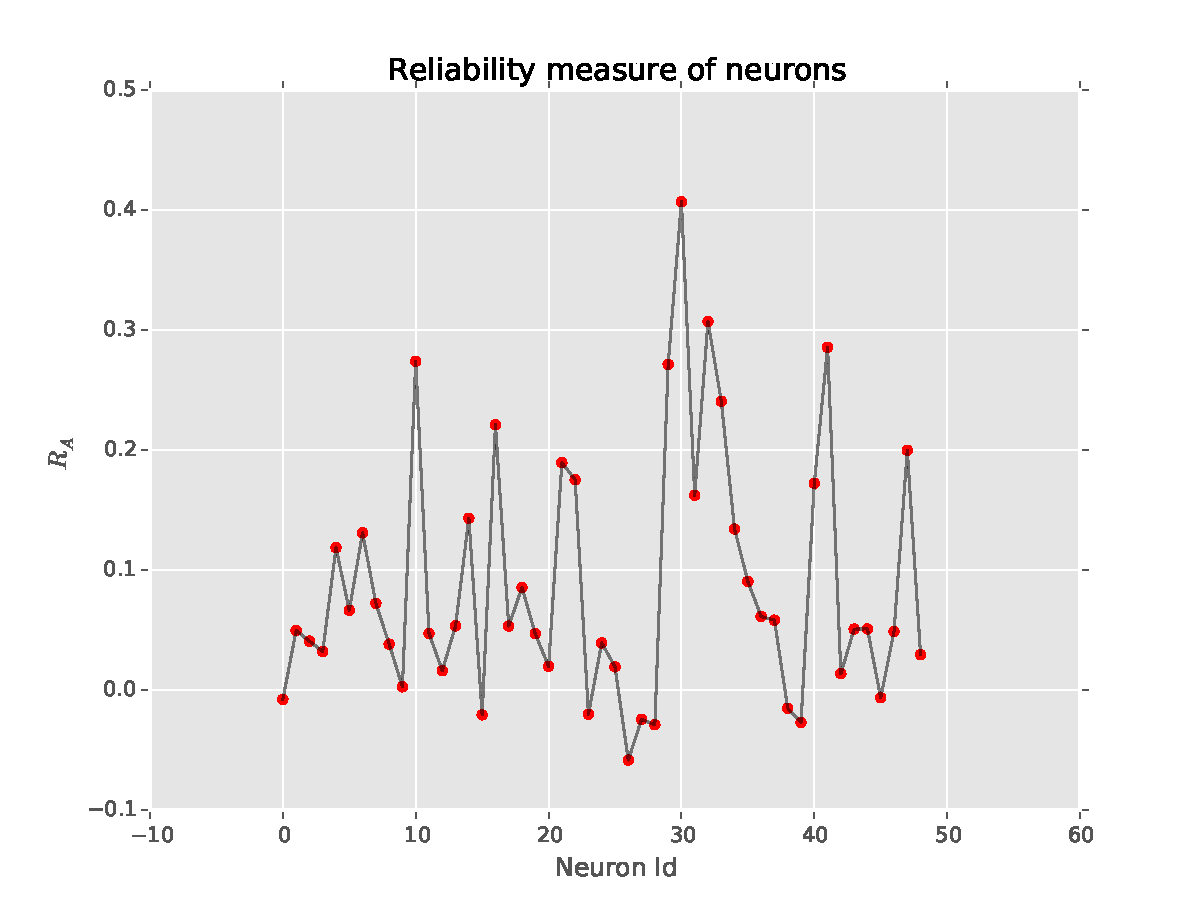
\includegraphics[width=.7\linewidth]{\plt/reliabMain_raPlot_2016_02_05_13_25_56.pdf}
    \caption{Reliability measure $R_A$ for different neurons}
    \label{img:ra}
\end{figure} 
% section study_of_reliability (end)
% section finding_similarly_tuned_neurons (end)
%%%%%%%%%%%%%%%%%%%%%%%%%%%%%%%%%%%%%%%%%%%%%%%%%%%%%%%%%%%%%%%%%%%%%%
\chapter{Searching for Motifs}       % 6 pages
\label{chap:searchmotif}
In Music, motif is a perceivable recurring fragment. They are elementary signatures that repeats to form bigger units. Detecting such motifs in a song tells us more about the song like its melody. In Genetics, motif is a sequence pattern of nucleotides in a longer DNA sequence. From a signal processing perceptive, motifs is a signal segment that recurs in a longer signal. A valid motif should have an `acceptable' length such that it has a significance. Motif analysis is import because in every domain, occurrence of motifs has a meaning to it.

In the experiment, each neuron responses are captured as a time series sampled at 20Hz for 10 seconds. In neuron responses we define a Motif as subsequence of response time series which has the following properties:
\begin{itemize}
   \item Recurs in the same response signal but in a different part \textbf{or}
   \item Recurs in the response of the same neuron to a different trial \textbf{or}
   \item Recurs in the response of another neuron in the same mouse \textbf{or}
   \item Recurs in the response of neuron in a different mouse \textbf{and}
   \item Has a significant length in time.
\end{itemize}
Analyzing motifs in neuronal signals will help us understand reliable information representation. Even if two responses of same trial has a long subsequence but not time synchronized, Study of reliability in Section~\ref{sec:study_of_reliability} will fail as the Pearson correlation coefficient will output a small value. Motivic analysis can detect such subsequences even if they are time shifted.

Study of motifs across two different neurons within a mouse can explain correlation between two neurons. Correlated neurons can represent neuronal interconnections. Correlated and synchronous activity in populations of neurons has been observed in many brain regions and has been shown to play a crucial role in cortical coding, attention, and network dynamics [\cite{rosenbaum2014correlated}]. Studying correlations between neurons is again not effective if they are time separated as Pearson correlation will fail. Analyzing motifs across neurons will be a better way to study neuronal correlations.

Motifs found in neurons from two \textit{different} mices will represent similar biological process both the neurons undergoes. As the motifs found cannot be due to interconnections, they are due to same activation mechanism of neurons. In this case, we would expect a small motif compared to motifs found within mouse.

In this chapter, we will analyze the presence of motifs in neuronal signals. The presence of motifs will motivate us to extract the motifs and their significance.
\section{Study of Autocorrelation Function (ACF)} % (fold)
\label{sec:study_of_autocorrelation_function_}

% section study_of_autocorrelation_function_ (end)
\section{ACFGram} % (fold)
\label{sec:acfgram}

% section acfgram (end)

%%%%%%%%%%%%%%%%%%%%%%%%%%%%%%%%%%%%%%%%%%%%%%%%%%%%%%%%%%%%%%%%%%%%%%
\chapter{Rough Longest Common Subsequence}     % 12 pages
\label{chap:rlcs}

%%%%%%%%%%%%%%%%%%%%%%%%%%%%%%%%%%%%%%%%%%%%%%%%%%%%%%%%%%%%%%%%%%%%%%
\chapter{Inferences and Future work}    % 3 pages
\label{chap:summary}

%%%%%%%%%%%%%%%%%%%%%%%%%%%%%%%%%%%%%%%%%%%%%%%%%%%%%%%%%%%%%%%%%%%%%%
\appendix
\chapter{Neural visual pathway}

%%%%%%%%%%%%%%%%%%%%%%%%%%%%%%%%%%%%%%%%%%%%%%%%%%%%%%%%%%%%%%%%%%%%%%
% Bibliography.
\pagebreak
\begin{singlespace}
  \begin{small}
	\bibliography{refs}
  \end{small}
\end{singlespace}
%%%%%%%%%%%%%%%%%%%%%%%%%%%%%%%%%%%%%%%%%%%%%%%%%%%%%%%%%%%%%%%%%%%%%%
\end{document}
